\phantomsection
\chapter{Feature Detection with Viola-Jones}
\label{chap:implementation_violajones}

\noindent The feature detection part for this Facial Expression Recognition system is based on the Viola-Jones face detection algorithm. This chapter describes how this Viola-Jones algorithm is used and implemented.
\newline

\phantomsection
\section{Viola-Jones}

\vspace{\baselineskip}
\noindent To apply Viola-Jones, video sequences of face are obtained thanks to a webcam or to the Kinect. Then the algorithm is able to detect face and regions of interest in the frames. The regions of interest are the nose, the left eye, the right eye and the mouth. 
\newline

\noindent Classifiers are trained prior to be used. Then they are loaded; one for the face and one for each region of interest. Then based on these classifiers, face and regions of interest are detected in the frames. Figure~\ref{violajones_implementation_example} shows an example of face detection. Some regions of interest are also detected. These regions are the mouth, the left eye and the right eye.
\newline

\begin{figure}[!h]
\begin{center}
\noindent 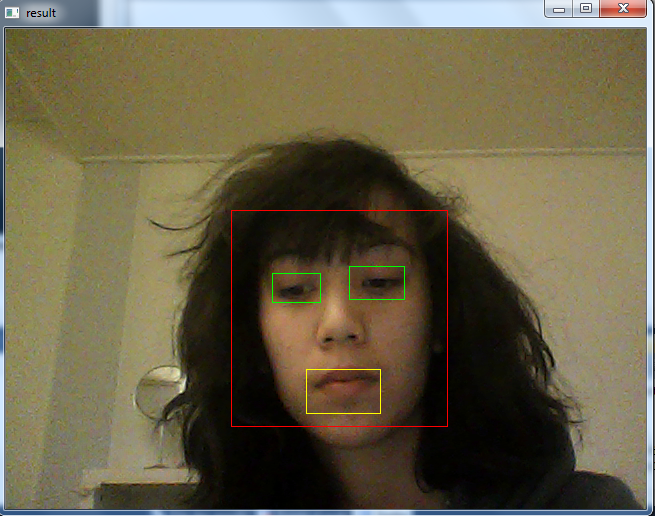
\includegraphics[scale=0.4]{figures/violajones_implementation_example} 
\newline
\caption{Example of face detection with Viola-Jones}
\label{violajones_implementation_example}
\end{center} 
\end{figure}